\section{Gestion des tournois}

\textbf{Si vous êtes membres du staff, et que vous avez la permission de gérer les tournois}, vous pouvez alors accéder à la page de gestion des tournois, depuis l'onglet "Staff" tout à droite du menu de navigation.

\begin{figure}[H]
\centering
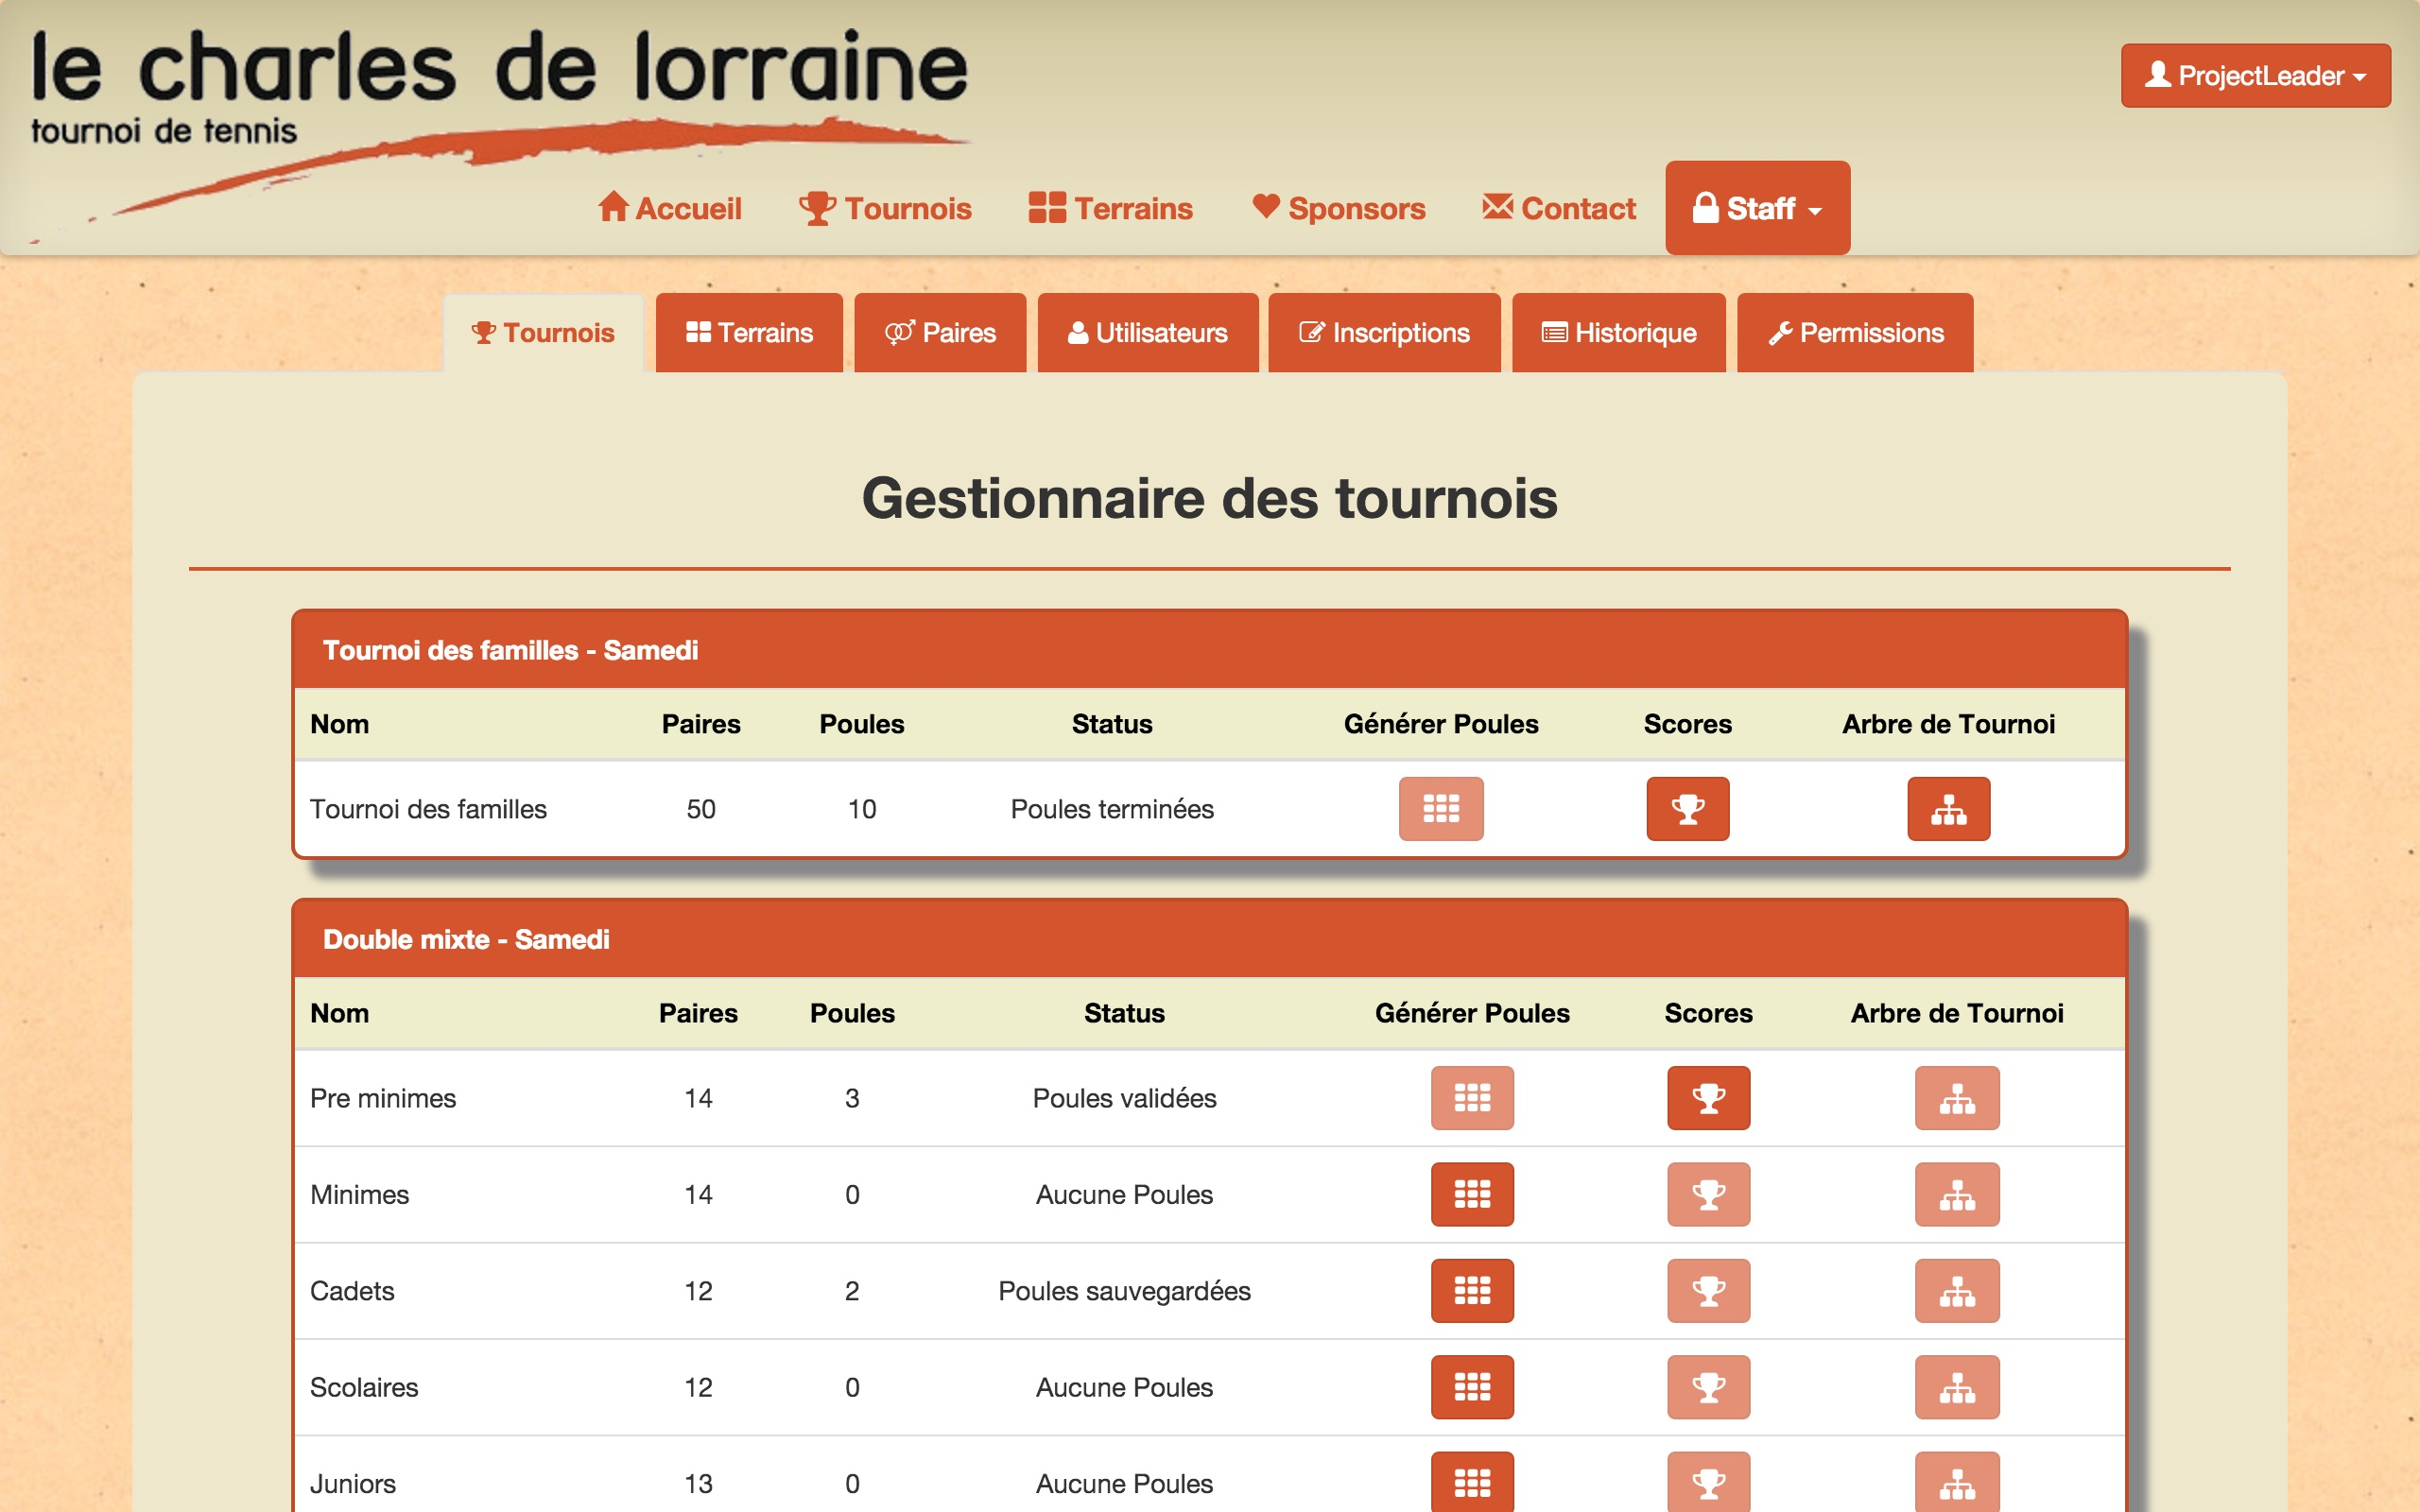
\includegraphics[scale=0.15]{gestion-tournois/gestion-tournois.jpg}
\caption{Page de la gestion des tournois}
\end{figure}

\subsection{Les tournois}

Depuis la page staff "Gestionnaire des tournois", vous pouvez gérer tous les tournois et catégories dont vous avez eu préalablement la permission de gérer. Pour donner la permission à un utilisateur de gérer certains tournois, l'admin doit lui octroyer les permission à partir de la page "Gestionnaire des permissions".
% TODO
\todo[inline]{Ajouter une référence vers la page Gestionnaire des permissions}

Sur cette page, vous pouvez consulter une liste de tournois. Les tournois sont catégorisés en fonction du type du tournoi :

\begin{itemize}
\item Tournoi des familles
\item Double mixte
\item Double hommes
\item Double femmes
\end{itemize}

\begin{figure}[H]
\centering
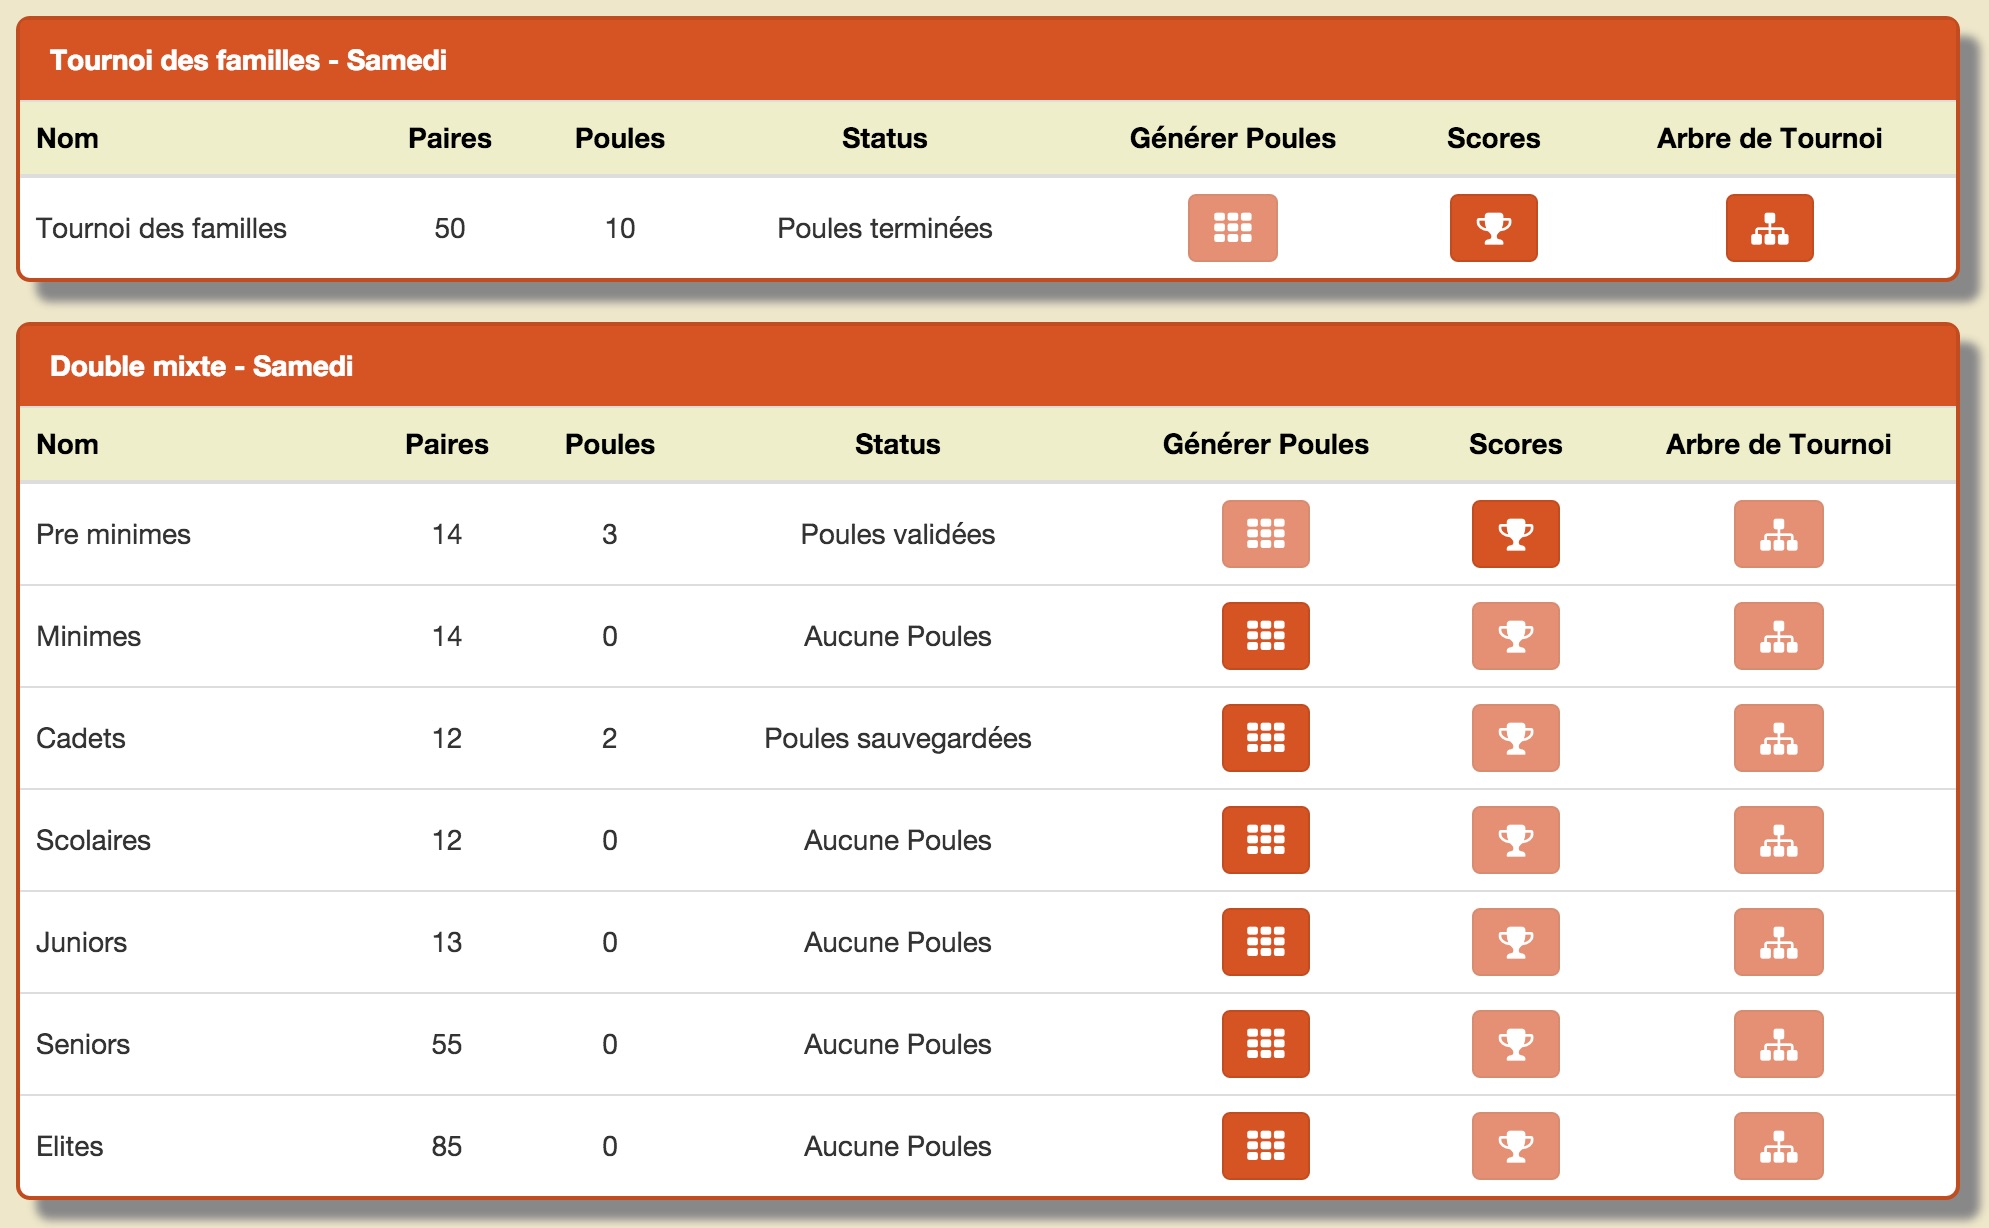
\includegraphics[scale=0.15]{gestion-tournois/gestion-tournois-liste.jpg}
\caption{Page de la gestion des tournois - liste des tournois}
\end{figure}

Tous les tournois, sauf le Tournoi des familles, sont à nouveau catégorisés en fonction de l'âge des joueurs. Ces sous-tournois sont ordonnés du tournoi des plus jeunes (Pré-minimes), au plus âgés (Élites).\newline

Chaque tournois indique les informations les plus importantes, à savoir :

\begin{itemize}
\item le nombre de paires inscrites
\item le nombre de poules actuel
\item le status du tournoi
\end{itemize}
\bigskip
L'état du tournoi impose les opérations possibles sur le tournoi. Par exemple :

\begin{itemize}
\item  \textbf{Aucune poules} n'autorise que de générer les poules ;
\item \textbf{Poules validées} permet d'encoder les scores ;
\item \textbf{Poules terminées} permet de consulter les poules, et de créer l'arbre d'élimination.
\end{itemize}
\bigskip
Il y a 3 pages de gestion des tournois, selon le status de celui-ci :

\begin{itemize}
\item \textbf{Générer Poules} : permet de créer, modifier, et sauvegarder les poules
\item \textbf{Scores} : permet de consulter les poules crées, supprimer les poules, imprimer les score boards, et encoder les scores de chaque poule
\item \textbf{Arbre de Tournoi} : permet de créer l'arbre du tournoi, imprimer l'arbre d'élimination, et encoder les scores dans l'arbre d'élimination
\end{itemize}

\begin{figure}[H]
\centering
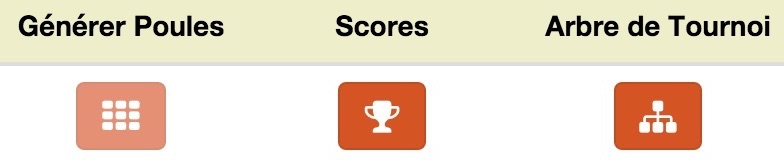
\includegraphics[scale=0.35]{gestion-tournois/gestion-tournois-operations.jpg}
\caption{Page de la gestion des tournois - accès aux pages spécifique de gestion}
\end{figure}

\subsection{Les poules}

\subsection{L'arbre d'élimination}